\section{Convolutional Neural Networks for Pedestrian Detection}

\subsection{CNN}
\begin{frame}{Convolutional Neural Networks}
  \centering
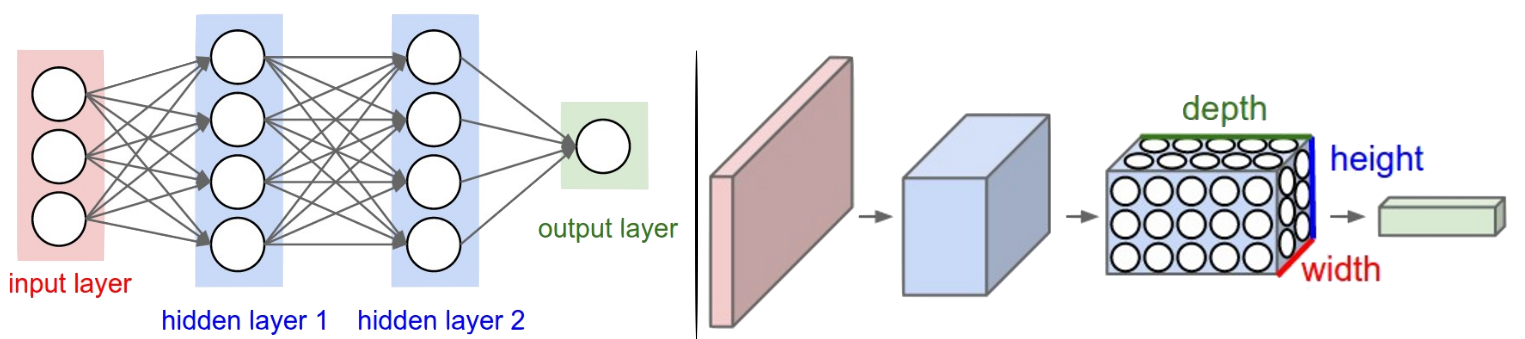
\includegraphics[width=\textwidth]{CNN.png}\\
\small
\vspace{1mm}
Neural Network \hspace{1.75cm} Convolutional Neural Networks
\end{frame}

\begin{frame}{CNN Layers}
  A CNN is made of different layers:
  \begin{itemize}
    \item \textbf{Convolution}
    \item \textbf{Non linearity (ReLU)}
    \item \textbf{Pooling}
    \item \textbf{Fully-Connected}
  \end{itemize}
  Many combinations have been proposed
\end{frame}

\begin{frame}{Convolution Layer}
\only<1>{
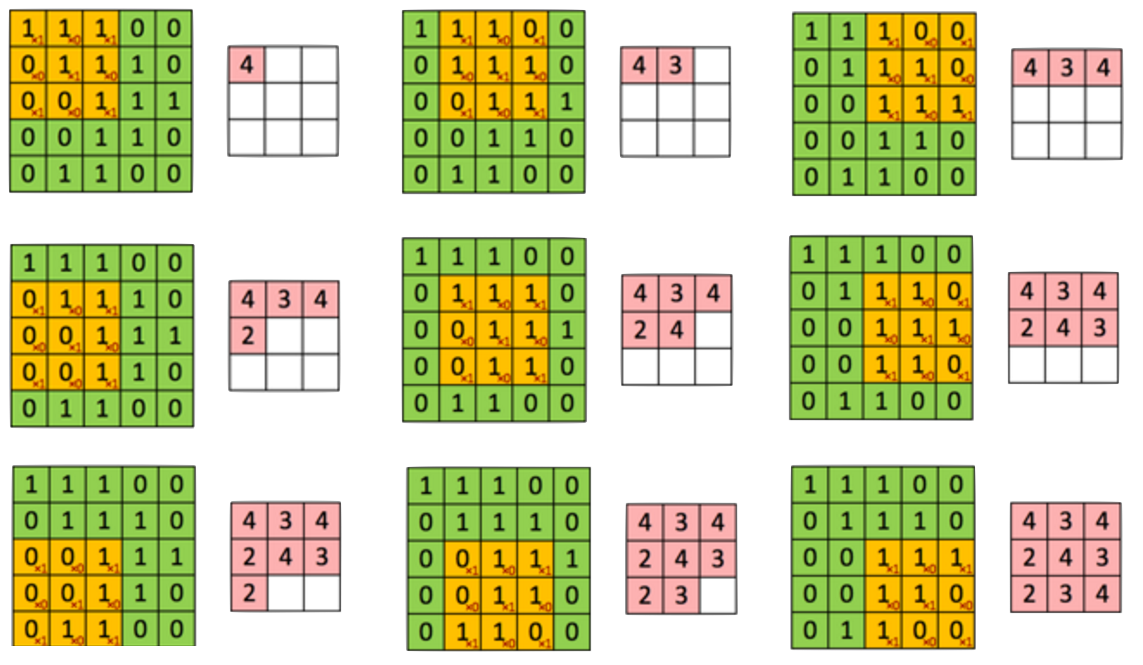
\includegraphics[width=\textwidth]{convolution.png}
}
\only<2>{
Extracts features from the input image\\
\vspace{1mm}
Preserves the spatial relationship between pixels\\
\vspace{1mm}
Convolution matrix also called \textit{filter}, \textit{kernel} or \textit{feature detector}\\
\vspace{1mm}
Output: \textbf{feature maps}\\
\vspace{1mm}
Different filters generate different feature maps\\
\vspace{1mm}
Filters' values learned during the training\\
}
\only<3>{
How many convolution matrices? $\rightarrow$ Number of filters or depth\\
\vspace{2mm}
Size of convolution matrices? $\rightarrow$ Depth\\
\vspace{2mm}
Step between each convolution? $\rightarrow$ Stride\\
\vspace{2mm}
Zero-padding for convolution on the border?
}
\end{frame}

\begin{frame}{Pooling Layer}
\only<1>{
  Downsampling operation (Max, Average, Sum etc.)\\
  Reduces the dimensionality of each feature map\\
  Retains the most important information\\
\vspace{10mm}
\begin{center}
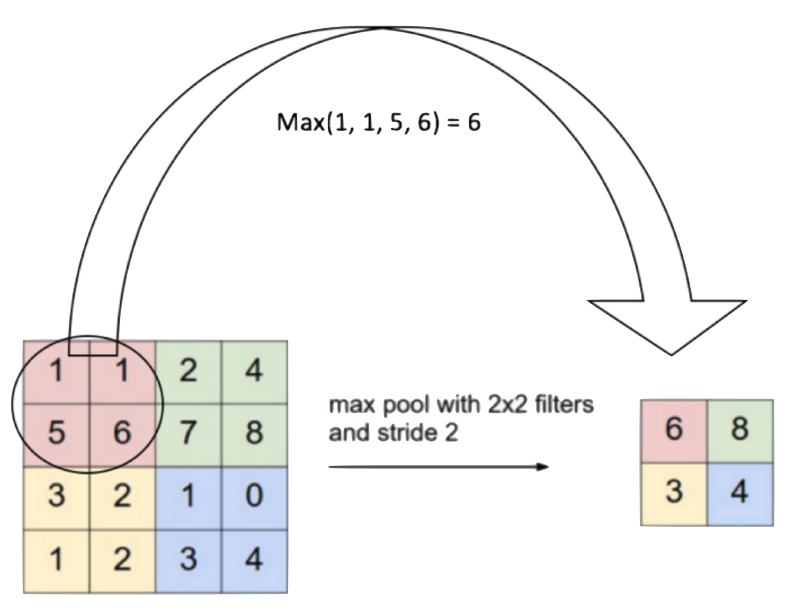
\includegraphics[width=.5\textwidth]{polling.png}
\end{center}

}
\only<2>{
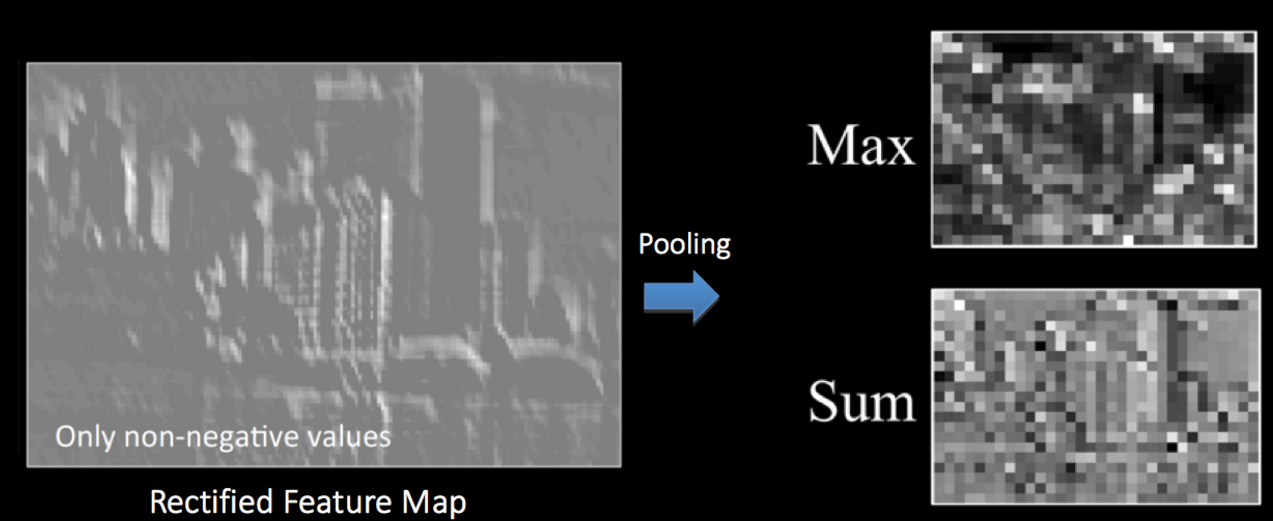
\includegraphics[width=\textwidth]{polling_example.png}
}
\end{frame}

\begin{frame}{Fully-Connected Layer}
  Classification operation\\
  \vspace{2mm}
  Traditional Multi Layer Perceptron\\
  \vspace{2mm}
  Computes the class scores\\
  \vspace{2mm}
  Examples: softmax activation function, SVM

\end{frame}
\subsection{DeepPed}
\begin{frame}{DeepPed}
  Improving and adapting AlexNet to pedestrian detection\\
  \vspace{2mm}
  Low miss rate (MR), about $19.9\%$\\
  \vspace{2mm}
  Not real-time, only 2 fps\\
  \vspace{2mm}
  Model:
  \begin{itemize}
    \item Locally Decorrelated Channel Features (LDCF)
    \item Data preprocessing
    \item Fine-tuned CNN
    \item SVM (using LDCF scores)
  \end{itemize}
\end{frame}

\begin{frame}{Data Preprocessing}
  \small
\only<1>{
  \textbf{Padding} to overcome the issue of imprecise proposed region:\\
  \begin{itemize}

      \item[-] \texttt{For each box of the training select the closer candidate region}
      \item[-] \texttt{Compute the padding needed so that the box is contained in the region}
      \item[-] \texttt{Build the histogram of the padding quantities and use the mean value}
  \end{itemize}

  %\texttt{
  %- For each box of the training select the closer candidate region\\
  %- Compute the padding needed so that the box is contained in the region\\
  %- Build the histogram of the padding quantities and use the mean value\\}
  \begin{center}
    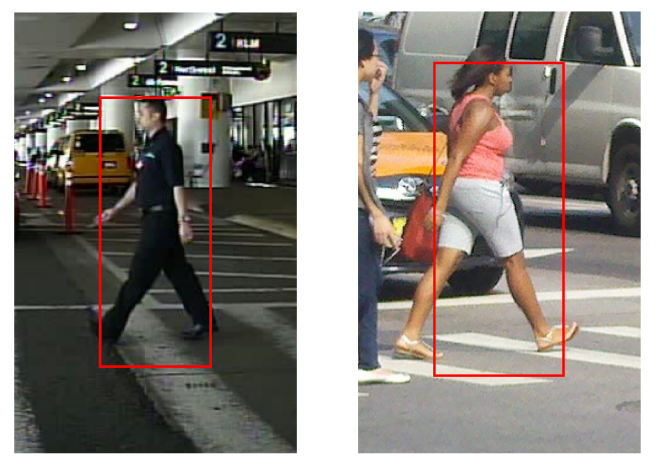
\includegraphics[width=.5\textwidth]{data_preproc.png}
  \end{center}
}
\only<2>{
  \textbf{Negative Sample Decorrelation}:\\
  \begin{itemize}
  \item[-] \texttt{Selects negative training examples that are as diverse as possible}
  \item[-] \texttt{Randomly extract N regions not containing a pedestrian}
  \item[-] \texttt{Compute their color histogram}
  \item[-] \texttt{Normalize it to obtain a probability distribution}
  \item[-] \texttt{Compute the euclidean distance between each pair of distribution}
  \item[-] \texttt{Select the furthest K regions}
  \end{itemize}
}

\end{frame}

\begin{frame}{Fine-tuned CNN}
  6 sessions as training set, 5 as test set\\
  \vspace{2mm}
  k-fold cross validation procedure (k = 6)\\
  \vspace{2mm}
  Resampling the test set (1 image every 30 frames) to reduce correlation\\
  \vspace{2mm}
  3000 iterations for the training procedure\\

\end{frame}

\subsection{DeepCascade}
\begin{frame}{DeepCascade}
  \small
  Improving and adapting AlexNet to pedestrian detection\\
  Good accuracy: MR = $26.2\%$\\
  \textbf{Real-time}: 15 fps\\
  Cascade model:
  \begin{itemize}
    \item frequently used method for \textbf{speeding up} classifiers
    \item divides classifiers into a sequence of \textbf{simpler classifiers}
    \item VeryFast cascade reduces recalls at each stage, increasing MR
    \item hybrid approach: use only 10\% of the stages in the cascade
  \end{itemize}
\end{frame}

\begin{frame}{DeepCascade - Model}
\small
\begin{enumerate}
  \item Pretraining
  \begin{itemize}
    \item pre-initialized weights based on Imagenet
    \item easy to incorporate and increases accuracy
  \end{itemize}

  \item Soft-cascade
  \begin{itemize}
    \item aborts the evaluation of non-promising detections
    \item hybrid approach uses 10\% of the stages of VeryFast
  \end{itemize}

  \item Tiny CNN classifier

  \item Modified AlexNet
  \begin{itemize}
    \item reduced depth and size
    \item faster
  \end{itemize}
\end{enumerate}
\end{frame}

\begin{frame}{Classifier and Detector}
  \small
\centering
  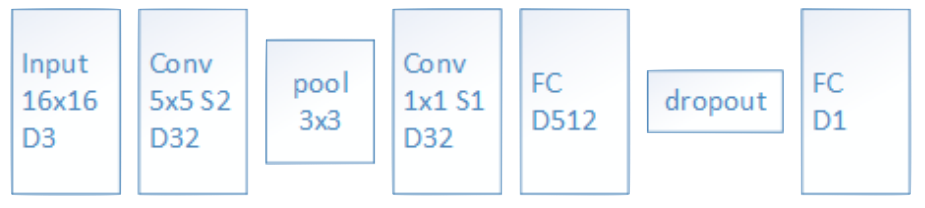
\includegraphics[width=.9\textwidth]{classifier.png}  \\
  The architecture of the tiny CNN classifier\\
  \vspace{1cm}
  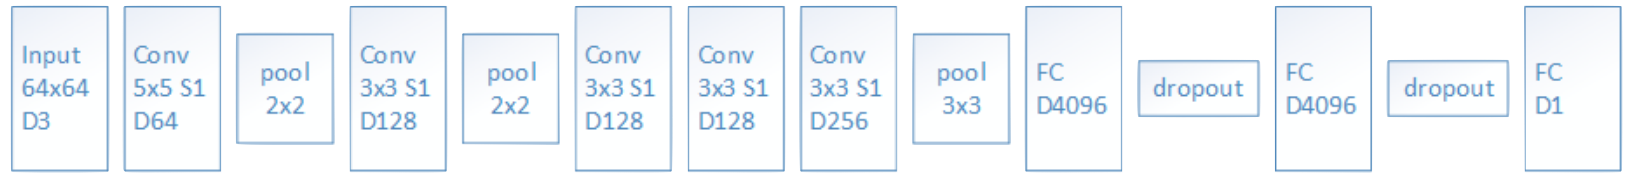
\includegraphics[width=.9\textwidth]{detector.png}  \\
  The architecture of the modified AlexNet
\end{frame}

\begin{frame}{Comparison}
  \centering
    \includegraphics[width=1\textwidth]{comparison.png}
\end{frame}
